\chapter{Fundamentals}
% \chapter{Fundamentals of Model-driven Software Engineering}
\label{ch:fundamentals}
In this chapter, the fundamentals of Model-driven Software Engineering are discussed. Moreover, we stress on fundamentals of Domain-specific Language and some DSL examples. Since this thesis focus on the migration of run-time states, we also give a categorization of applications states. Furthermore, as we use JSON to define our DSL, we discuss about JSON and JSON Schema.

\section{Model-driven Software Engineering}
The Model-driven software engineering (MDSE) methodology takes the premise that models, as crucial elements of understanding and sharing complex software, are a practical way of working and thinking by transforming them into first-class citizens in software engineering. The purpose of a model can be anything from communication between people to the ability to develop a piece of software. The actual needs that they will address will determine how a model is defined and managed. \cite{mdse}. 

\begin{definition}[Model \cite{mda-10.5555/579151}]
A model is essentially an abstract representation of a software system’s structure, function, or behavior. 
\end{definition}

The model indicates that parts of the software system are generated. However, it may also indicate that the model should be interpreted at run-time, making it a central artifact as part of the software development process.

\subsection{Model-driven Development (MDD)}
MDD refers to a development paradigm in which models are their primary artifact. In MDD, the implementation is usually generated from the models (semi)automatically\cite{mdse}. MDD increases development speed. This is achieved through the automatic code generation from a model with transformation steps. In MDD, when a software architectures are defined and implemented, automated transformations increase software quality, since consistency is emphasized\cite{mdsd_en}.
.

\subsection{Model-based Engineering (MBE)}
MBE or Model-based development is referred to as a softer version of MDE that models are not necessarily first-class citizens. The MBE process concerns the use of models in development, although they are not the key artifacts. As one example, consider a development process in which designers specify the domain models of the system during the analysis phase but then make the models available to programmers as the blueprints, to write the code without automatic code-generation involved \cite{mdse}.


\section{Domain-specific Language}
A Domain-Specific Language (DSL) is a language that is designed exclusively for a certain application domain. The language deals with the concepts and features specific to that particular domain. \cite{dsl}.
Following are the most vital points in a DSL. The notation by which users can write programs is specified in the \textit{concrete syntax}. This notation can be textual, visual, or a combination of these. A data structure containing semantically related information conveyed by a model is known as \textit{abstract syntax}. It is devoid of any knowledge about the notation. In addition to structurally sound in terms of concrete and abstract syntax, a language's \textit{static semantics} is the collection of constraints and/or type system rules that programs must follow. The interpretation of a program to execute is referred to as \textit{execution semantics} \cite{dsl-eng}.

\begin{definition}[Metamodel \cite{dsl-eng}]
The metamodel of a model is a model that defines the abstract syntax of a language used to describe a model. 
\end{definition}

In metamodel, the meta prefix can be interpreted as \textit{the definition of}. This model represents an \textit{instance of} the metamodel. It should be mentioned that metamodel itself also is a model.

\subsection{Define a DSL}
Designing DSLs accordingly requires careful attention to detail to meet requirements. Essentially, the main concern of DSL design consists of implementing concrete syntax and abstract syntax \cite{engineering_modeling_languages}.
 
There are some steps that they have to be considered for creating a DSL \cite{mdsd_en}.

\begin{enumerate}
\item Define DSL metamodel
    \item[] The metamodel should defines the abstract syntax and the static semantics of a DSL. The metamodel should be defined in way to prevent unwanted instances. In order to define a metamodel, a metamodeling language is required, which is described by a meta meta model. For example, in this thesis we use UML to define our metamodel which explained in 5.1.1.

\item Define concrete syntax
    \item[] Since the DSL is used as the ‘user interface’ for the metamodel, it is important that developers understand, write and interpret the models properly. Thereby, a suitable concrete syntax should be considered. As this thesis involves a textual language, we chose to use JSON, which is discussed in the next section.
\item Define the mapping between abstract syntax and concrete syntax
    \item[] There should be a proper mapping to map elements of the concrete syntax to the metamodel elements. For example, in this thesis we mapped our DSL's metamodel in JSON schema which discussed in 5.1.3.

\item Define DSL semantics
    \item[] The semantics are typically explained informally in natural language. A DSL's semantics must either be intuitively clear to the modeler or well-documented. One advantage of the DSL is its ability to adapt to concepts from the problem space so that domain experts will recognize its ‘domain language’.
\item Define model transformations and code generators
    \item[] Essentially, model transformations work like programs that take in models as input. Model transformations differ and are used in different ways, which can be expressed differently through their inputs and outputs. When a model is defined based on its metamodel, model transformation indicates which models can be accepted as input and, if appropriate, what models can be produced as output \cite{model_transformation}.
    \item[] The code generators are metaprograms that use specifications or models as input parameters and generate code as output.  Also, it should be defined which part will be generated, so the generated code can be separated from the manually-created code, and the developer must integrate both.

\end{enumerate}

\subsection{DSL Examples}
This section discusses two existing textual DSLs.

\subsubsection{Amazon States Language}
This language is a specification for state machines. These state machines are a collection of states that perform tasks. This specification allows the state machine to determine the transition to other states and stop the execution. These languages are used within the Amazon Web Services infrastructure, and they use lambda functions to execute tasks \cite{amazonwebservices}. Listing \ref{lis:asl} shows an simple example of Amazon States Language, which contains two states and starts from \textit{HelloWorld} state and have transition to \textit{NextState} and finishes there.

\FloatBarrier
\begin{code}
\begin{json}
{
    "Comment": "A minimal example of the Amazon States language",
    "StartAt": "HelloWorld",
    "States": {
        "HelloWorld": {
          "Type": "Task",
          "Resource": "aws:lambda:eu-west:function:HelloWorld",
          "Next": "NextState",
        },
        "NextState": {
          "Type": "Task",
          "Resource": "aws:lambda:eu-west:function:FunctionName",
          "End": true
        }        
    }
}
\end{json}
\caption{A simple example of the Amazon States language \cite{amazonstate}}
\label{lis:asl}
\end{code}
\FloatBarrier

\subsubsection{PlantUML}
PlantUML is an open-source DSL allowing users to define different kinds of UML diagrams from a textual language. For example, All UML diagrams in this thesis are generated from PlantUML.
Listing \ref{lis:plantuml} shows a simple UML sequence diagram in PlantUML syntax. Also Figure \ref{fig:plantuml} shows the generated graphic of Listing \ref{lis:plantuml}.

\FloatBarrier
\begin{code}
\begin{js2}
@startuml

autonumber

A -> B: step

activate B
B -> C: step

activate C
C --> C: action
C -> B: step
deactivate C

B -> A: step
deactivate B

@enduml
\end{js2}
\caption{A simple sequence diagram in PlantUML syntax}
\label{lis:plantuml}
\end{code}
\FloatBarrier

\FloatBarrier
\begin{figure}[H]
    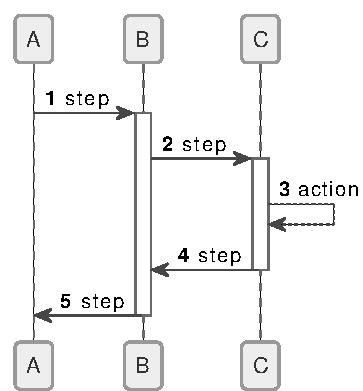
\includegraphics[scale=1]{../figures/example.pdf}
    \centering
    \caption{A generated simple sequence diagram in PlantUML}
    \label{fig:plantuml}
\end{figure}
\FloatBarrier

\section{Application State Space}
All possible combinations of an application are represented in a state space. Abstractions of state space are helpful when we want to comprehend the behavior of a given system. A state variable represents a particular state of the application; the values of all state variables describe the state of the application. This means each point in the state space represents one state of the application \cite{state-space}. The application states of existing applications are categorized in this thesis in order to identify those that can be migrated.

\paragraph{Persistent State}
A state that exist longer than a single execution of the program is considered to be a persistent state. In practice, the state is maintained by storing it as data in the computer's data storage \cite{pstate}. For example, the settings of the browser.


\paragraph{Action State}
A running application will frequently alter the run-time state due to processing, which is called an action state. For example, a browser is printing a page.

\paragraph{Run-time State}
In an application, variables represent the storage locations in the computer's memory that the computer uses to hold data stored. The run-time state of an application is the content of these memory locations at any point in its execution \cite{Laplante2000-ui}. For example, the value of a search input. In this thesis, the focus is on supporting the migration of such states.

\section{JSON}
JSON (JavaScript Object Notation) is a file format. It is lightweight and human-readable text to store and transmit data based on the data types of the JavaScript programming language \cite{json}. In the last few years, many programming languages support JSON, which gained popularity among developers, and has become the primary data format for exchanging information. JSON documents consist of key-value pairs, in which the value can be again a JSON object. Objects are key-value pairs. Each key is a string and denotes a property of the object. The value can be of a primitive data type (number, string, boolean, etc.), it can be an array of values or again an object, and there is no limit to the nesting level \cite{json-schema}. 

A simple JSON document is shown in Listing \ref{lis:json} which \textit{fullname} and \textit{email} are keys and \textit{"John Doe"} and \textit{"john@mail.upb.de"} are their string values. Moreover, \textit{info} is an object containing another key that is \textit{hobbies} contains an array value.

\FloatBarrier
\begin{code}
\begin{json}
{
    "fullname": "John Doe",
    "email": "john@mail.upb.de",
    "info" : {
        "hobbies" : ["watching movies", "wood carving", "football"]
    }
}
\end{json}
\caption{A simple JSON document.}
\label{lis:json}
\end{code}
\FloatBarrier

\section{JSON Schema}
After the huge popularity of JSON, certain scenarios could benefit from a declarative method for identifying a schema for JSON documents.
A declarative schema specification would give programming languages and developers a standardized language to specify what types of JSON documents are valid as inputs and outputs \cite{json-schema}.

The schema can be another JSON document that defines acceptable key-value pairs.
For instance, the simple JSON document in Listing \ref{lis:json}, can be declare in JSON Schema document in Listing \ref{lis:json-schema}.

\FloatBarrier
\begin{code}
\begin{json}
{
    "properties": {
        "fullname": {
            "type": "string"
        },
        "email": {
            "type": "string",
            "format": "email"
        },
        "info": {
            "type": "object",
            "properties": {
                "hobbies" : {
                    "type": "array"
                }
            }
        }        
    }
}
\end{json}
\caption{A simple JSON Schema document}
\label{lis:json-schema}
\end{code}
\FloatBarrier

JSON Schema can define a document must have several , including regular data-types like objects, arrays, strings, booleans, numbers and, null. Each of these types has different keywords that help to specify and restrict the schema. The most important attribute is “type” whose value is defining the schema. With validation keywords included in the schema, constraints can be applied to an instance. \cite{json-model}. For example in Listing \ref{lis:json-schema}, \lstinline[basicstyle=\ttfamily]|{"type": "string"}| specify a value with string type.

We use YAML syntax to represent the Application State Model in JSON Schema in this thesis for readability reasons. YAML is a human-readable syntax and can be converted to JSON syntax without extra configuration. Listing \ref{lis:yaml-simple} shows a simple example based on Listing \ref{lis:json-schema} which is a JSON Schema document.


\lstset{
  label=lis:yaml-simple, caption=Example of expressing JSON Schema in YAML syntax., 
}
\begin{lstlisting}[language=yaml]
properties:
  fullname:
    type: string
  email:
    type: string
    format: email
  info:
    type: object
    properties:
      hobbies:
        type: array
\end{lstlisting}

